%Formatting
\documentclass[12pt,a4paper]{book}
\usepackage{setspace} 
\doublespacing
\usepackage{float}
\usepackage[]{geometry}
\usepackage{xargs} 
\setlength{\parindent}{0in}
\restylefloat{table}
\usepackage{tcolorbox}

%Mathematics
\usepackage{amsmath}
\usepackage{amssymb}
\usepackage{mathtools}
\usepackage{graphicx}
\usepackage{float}
\usepackage{tocloft}
\usepackage{circuitikz}
%\usepackage[pdftex,dvipsnames]{xcolor}

%\definecolor{OliveGreen}
%\definecolor{Plum}

\definecolor{commentsColor}{rgb}{0.497495, 0.497587, 0.497464}
\definecolor{keywordsColor}{rgb}{0.541176, 0.168627, 0.886275}
\definecolor{stringColor}{rgb}{0.000000, 0.558215, 0.135316}
%Computer Science
\usepackage{listings}
\lstset
{ %Formatting for code
	basicstyle=\footnotesize\ttfamily,
	numbers=left,
	%caption={},
	%title={},
	stepnumber=1,
	showstringspaces=false,
	tabsize=1,
	breaklines=true,
	breakatwhitespace=false,
	frame=lines,
	xleftmargin=2em,
	framexleftmargin=1.5em,
	commentstyle=\color{commentsColor}\ttfamily,
  	stringstyle=\color{stringColor}\ttfamily,
	keywordstyle=\color{keywordsColor}\bfseries,
}
\newcommand{\lstprompt}{>>>}
\newcommand{\numberwithprompt}[1]{\footnotesize\ttfamily\selectfont \lstprompt}


% https://tex.stackexchange.com/questions/340232/how-insert-a-character-at-the-begin-of-every-line-from-a-source-code
\lstdefinestyle{console} {
	basicstyle=\footnotesize\ttfamily,
	numbers=left,
	stepnumber=1,
	showstringspaces=false,
	tabsize=1,
	breaklines=true,
	breakatwhitespace=false,
	frame=single,
	xleftmargin=2em,
	framexleftmargin=2.5em,
	%backgroundcolor=\color{gray!55},
	numberstyle=\numberwithprompt,
	}

% \lstdefinelanguage{psuedocode}{
%   keywords={typeof, new, true, false, catch, function, return, null, catch, switch, var, if, in, while, do, else, case, break},
%   keywordstyle=\color{blue}\bfseries,
%   ndkeywords={class, export, boolean, throw, implements, import, this},
%   ndkeywordstyle=\color{darkgray}\bfseries,
%   identifierstyle=\color{black},
%   sensitive=false,
%   comment=[l]{//},
%   morecomment=[s]{/*}{*/},
%   commentstyle=\color{purple}\ttfamily,
%   stringstyle=\color{red}\ttfamily,
%   morestring=[b]',
%   morestring=[b]"
% }

\usepackage{algpseudocodex}
%Book Stuff
\newenvironment{dedication}
{%\clearpage           % we want a new page          %% I commented this
	\thispagestyle{empty}% no header and footer
	\vspace*{\stretch{1}}% some space at the top
	\itshape             % the text is in italics
	\raggedleft          % flush to the right margin
}
{\par % end the paragraph
	\vspace{\stretch{3}} % space at bottom is three times that at the top
	\clearpage           % finish off the page
}

%Citations
%\usepackage{cite}
\usepackage[backend=bibtex,style=verbose-trad2]{biblatex} %works really really well, but no MLA format
% %\usepackage[backend=biber,style=mla]{biblatex} %Doesn't print all sources for some reason
\usepackage{caption}
\captionsetup[lstlisting]{font={small,tt}}
\newcommand{\source}[1]{\caption*{Source: {#1}} }

\bibliography{references.bib} 

\newcommand{\listequationsname}{List of Equations}

%Symbols and Other
\newcommand{\figref}[1]{Fig. \ref{#1}}
\newcommand{\coderef}[1]{Code Ex. \ref{#1}}
\newenvironment{codex}{begdef}{codex} % Define example here
\usepackage{upgreek}
\usepackage{hyperref}
\hypersetup{
	colorlinks,
	citecolor=black,
	filecolor=black,
	linkcolor=black,
	urlcolor=black
}

% Drafting Stuff (CHANGE FOR FINAL) TODO [!!!]
\usepackage[colorinlistoftodos,prependcaption]{todonotes}
\usepackage{draftwatermark}
\usepackage{lipsum}

\SetWatermarkText{\texttt{DRAFT}}
\SetWatermarkScale{7}
\SetWatermarkAngle{45}

\newcommandx{\unsure}[2][1=]{\todo[linecolor=red,backgroundcolor=red!25,bordercolor=red,#1]{#2}}
\newcommandx{\change}[2][1=]{\todo[linecolor=blue,backgroundcolor=blue!25,bordercolor=blue,#1]{#2}}
\newcommandx{\toadd}[2][1=]{\todo[linecolor=green,backgroundcolor=green!25,bordercolor=green,#1]{#2}}
\newcommandx{\info}[2][1=]{\todo[linecolor=yellow,backgroundcolor=yellow!25,bordercolor=yellow,#1]{#2}}
\newcommandx{\improve}[2][1=]{\todo[linecolor=pink,backgroundcolor=pink!25,bordercolor=pink,#1]{#2}}
\newcommandx{\hiddentodo}[2][1=]{\todo[disable,#1]{#2}}

\begin{document}
	\title{java.util.helpmepls; \\
	if \_\_name\_\_ == ``\_\_pain\_\_:'' \\
	\large{\textit{Learning to Code from a Subpar Programmer}}}
	\author{Aditya K. Rao}
	\date{\texttt{Work in progress \\ Last Edited: \today}}
	\maketitle

	\begin{dedication}
		``For anyone that wants to learn how to code or something''
		%``Dedicated to Arnav's fat juicy ass''
		\par   %% or a blank line
		%\vspace{2\baselineskip}
		
		\vspace{\baselineskip}
		%\usefont{T1}{LobsterTwo-LF}{bx}{it}
		- Adi
	\end{dedication}
	
	\tableofcontents
	\listoftodos
	TODO KEY [\textbf{IGNORE}]\unsure{Review work and see if it needs to change}\change{Make changes to existing work}\toadd{Add something is missing}\info{Expand upon exisitng work}\improve{Rewrite or reword to improve existing work}

	%\begin{abstract}
	%\end{abstract}
	%\textit{For all those people who asked me what course I used to learn how to code, I hope this helps make your journey easier}
	
	%\newpage
	\chapter*{Prologue/Introduction}  \label{chap:intro}
		Hi there, my name is Adi. At the time of writing this book, I recently have graduated from highschool and am on my way to university soon. Over the last four or five years, I've developed a deep interest in the ever elusive world of code. My main language is Python but I've recently diversified into many other avenues like Java, JavaScript, HTML, CSS, C++, Dart, and a few others. However, Python is definitely the language I have the most experience in. As such, that will be the basis for most of the actual code snippets in this book. I will also provide a few examples in psuedocode whenever I do something in a certain language. \change{Potentially rewrite, sounds litte childish?}
		\\\\
		I don't consider myself to be any authority on Computer Science/Engineering or anything like that, I'm just a guy who thinks he's got a decent method to help some people pursue their interests. My objective with this book is not really to help you learn a certain language, rather, it gives you the tools and knowledge to help you learn whatever language you want.\unsure{Maybe not the best in the introduction, consider rewriting}
		\\\\
		Many people who want to learn how to code already have an objective in mind and simply want the tools to make that dream a reality. Others just are interested in the subject area as a whole, some just want to get ahead of the curb and learn the skills required in a world ever dominated by tech. All of these are valid reasons for someone to learn to code. However, there is a difference between a person who knows how to program, and a programmer. Thea former can give instructions to a computer and knows what to expect as an output. The latter knows how and why a computer is doing what it is doing to make their instructions more and more efficient
		\\\\
		Therefore, these are the topics that we'll delve into in this instructional guide. First, we'll start with why you should be interested in code. Next, we'll progress into what coding actual is. Then, we'll take a turn and look at the inner workings of a computer and what components like the CPU and RAM actually do and how a computer understands the instructions that you give it. Then we'll learn some of the basics of any major high-level programming language (examples will be given in \textit{Python, Java, and psuedocode}) and techniques to go along with it. Lastly, we'll go into some of the most important skills for a coder, the way you need to think about problems. This is by far the most important - and one of the most overlooked - skills that you develop when programming.
		\\\\
		From there, we'll go over the future and some good resources to look at to progress your skills past what you have been taught here. Good luck on your coding journey.

	\chapter{Why learn how to code}  \label{chap:why-code}
		There are a variety of reasons why one would want to learn how to code. First and foremost, ever second, there are millions of developers around the world trying to automate something new. Everyone is searching for problems to try and solve - every hour of every day. That means that by not learning how to code, you may be putting yourself on the back-foot as it's a skill more and more employers are looking for in candidates.
		\section{Interest}
			For a lot of us, personal interest is what's motivating us to learn how to code. You could be intrigued by the software side and how a machine can be controlled and worked with to do what you want. Essentially, we wanted to see how we make a computer go bleep bloop using words.
		\section{Education}
			You may be looking for a new route in your education career. Coding is a skill that can help you in almost any field. Even something like history where you almost definitively will not be writing any code, skills like Decomposition will help you breakdown your tasks and methodically complete them. 
		\section{Freedom}
			The last opportunity that coding gives you is freedom. In our technology enhanced world almost everything is in some way shape or form dependent on some sort of tech. If you want to start a business or some sort of initiative, tech skills can help you start your concept, be a better manager by understanding the work being conducted, or by simply allowing you to automate monotonous tasks giving you more time to do what you want. \change{This section is written a bit poorly}

	\chapter{What is coding?}  \label{chap:intro-coding}
		What actually is coding? Many people don't seem to understand what someone who  codes actually does. We've all seen those scenes in movies and TV shows where the protagonist (or antagonist) says a bunch of tech words, sometimes throws a "quantum" or two in there for good measure, and then how is able to stop a software nuke (whatever that is) from annihilating downtown Brooklyn. It's not nearly as glamours. When you code, you're simply giving instructions that a machine can understand and execute.
		\\\\
		Now, the machine doesn't actually understand the words you write, instead it translates them into machine code/language. This is essentially a giant list of Ones and Zeros which the computer can use to turn switches off and on. That's basically how a computer works - turning switches off an on - zero and one.
		\\\\
		By manipulating these switches, we as programmers are able to make the computer do what we want. However, it would be incredibly laborious and confusing to type out said 1s and 0s by hand - though this was done using ``punch cards'' in the early days of the computer. Instead, we write code in what are known as ``high-level languages.'' These essentially make it easier for people to read and write code, allowing a machine to convert the words (aka syntax) into machine code.
		\\\\
		That is all that coding is, giving a machine a set of instructions and hopeing it does what you want. My friend likes to joke around, saying that ``Computer Science should be considered an experimental science'' because it can be mostly trial and error at times as you try to figure out how something works. 
		\\\\
		There are a few different types of coders: front-end and back-end. There are of course a few other flavors - i.e. mobile and game development - but these are the two most prominent ones. By no means do you have to stick to one once you choose it, but the skill sets for each are quite different. A front-end developer are generally people who focus on the \textbf{user experience} aka \textbf{UX} and \textbf{user interface} aka \textbf{UI}. If you're look at a website, that's typically the work of a front-end developer. On the flip side, we have back-end developers. Back-end developers are responsible for delivering content and internal logic of how some system works. For example, if you login to a website the process by which your account is authenticated and validated is the work of a back-end developer.

	\chapter{How does a computer work?}  \label{chap:computers}
		Knowing how a computer works is what separates the good from the great. When you understand how a computer works you, it's easier to make code more efficient and understand how your code works on the lower-levels (machine and assembly language).
		\section{Ones and Zeros} \label{sec:computers-binary}
			When you write code, you're essentially writing a bunch of words which get turned into 0s and 1s. These 0s and 1s subsequently are used to tell the computer whether to turn a switch on or off (also known as high or low as if the switch is \textit{on} then a \textit{higher} current is sent across the wire and vice versa). This number system is known as \textit{binary} or \textit{base-2}. On the other hand, our number system is called \textit{decimal} or \textit{base-10} because we have 10 digits (0, 1, 2, 3, 4, 5, 6, 7, 8, and 9).
			\subsection{Binary}
				Binary only has two digits - hence base-2 - which are 0 and 1. Each place value is a multiple of 2 with the first being $2^{0}=1$, then $2^{1}=2$, $2^{2}=4$, $2^{3}=8$ and so on as can be seen in Table \ref{tab:binary1}.
				\begin{table}[H]
					\centering
					\label{tab:binary1}
					\begin{tabular}{c||c|c|c|c|}
						\textbf{Decimal Value} & 8 & 4 & 2 & 1 \\
						\hline
						\textbf{Binary Value} & & & & 
					\end{tabular}
				\end{table}	
				To write a number from decimal to binary you simply take the biggest possible number from left to right. For example, if I have 11, first I'd subtract: $11-8=3$ since $11\geq8$and then add a 1 under the 8 in place value. Then I'd check if $3\geq4$ - since that's false, we add a 0 underneath 4 in place value and move to the next digit. We check if $3\geq2$, which is true, therefore we $3-2=1$. Finally we end by checking if $1\geq1$ if it is, then we add a 1 in the ones place. This can be seen in Table \ref{tab:binary2}:
				
				\begin{table}[H]
					\centering
					\label{tab:binary2}
					\begin{tabular}{c||c|c|c|c|}
						\textbf{Decimal Value} & 8 & 4 & 2 & 1 \\
						\hline
						\textbf{Binary Value} & 1 & 0 & 1 & 1 \\
					\end{tabular}
				\caption{ \\
					\textit{Decimal Number:} \textbf{11} \\ \textit{Binary Number:} \textbf{1011}}
				\end{table}	
				
				An alternative method is you keep dividing by 2. If you get the remainder as 0, you add a 0 to your number, if you get a 1, you add a 1 (don't change the number you're diving by). Lastly, you write the entire number our backwards. This can be illustrated in Table \ref{tab:binary3} below with 29:
				\begin{table}[H]
					\centering
					\label{tab:binary3}
					\begin{tabular}{c|c}
						\textbf{Working} & \textbf{Remainder} \\
						\hline
						$29\div2=14$ & 1 \\
						$14\div2=7$ & 0 \\
						$7\div2=3$ & 1 \\
						$3\div2=1$ & 1 \\
						$1\div2=0$ & 1 \\
					\end{tabular}
					\caption{ \\
						\textit{Decimal Number:} \textbf{29} \\ \textit{Binary Number:} \textbf{11101}}
				\end{table}	
				
			Now in Computer science we have a few terms for certain sets of data. A single digit is called a bit. If we have a binary number that's 4 bits, it's called a \textit{nibble}; if it's 8 bits long, it's a byte. From here it's easier to understand. 1024 bytes= 1 kibibyte (KiB). \textbf{However,} this is only if we're being extremely technically accurate. Generally 1024 bytes is taught - and learned - as a kilobyte (kB); in reality a kilobyte is actually 1000 bytes (hence kilo). 1024 KiB = 1 MiB (Mebibyte) 1000 kB = 1 MB (Megabyte) and so on.
				\\\\
			I additionally want to add some general information that can be useful in your everyday life. There's a difference between KiB, kB, and kb (and MiB, MB, and Mb and others). The first is a \textbf{Kibibyte} which is 1024 bytes. The second is a Kilobyte which is 1000 bytes. The last is 1024 \textit{\textbf{bits}} \textbf{not} \textit{bytes}. Internet service providers like to use this trick to make their speeds seem faster than they actually are - specifically with kB and kB (or MB and Mb). Computer/Mobile manufactures do something similar with KiB and kB (MiB and MB) to make it seem like their devices have more storage than they do. 
				\\\\
				There are more complex things in binary, such as binary addition, subtraction, multiplication, and division. However, I don't think it's really necessary or practical most of the time. If you're interested, I recommend taking a look at this video \toadd[inline]{Add in video here}
			
			\subsection{Alternative Number systems}
			Alternatively, hexadecimal - base-16 - is commonly used as a representation for binary numbers as it can easily be used to show nibbles with a single character. Hex has 16 digits (0, 1, 2, 3, 4, 5, 6, 7, 8, 9, A, B, C, D, E, and F). This means we can represent any byte with two digits. This is quite convenient whenever we do need to look at the raw binary of some data.
				\\\\
			An example of 255 in hexadecimal is FF. You can quickly convert between decimal and hex by multiplying each place value by the corresponding power of 16. For example, AF is $10\times16^{1}+15\times16^{0}=160+15=175$. If you want to convert decimal to hex, I find the easiest way is first to convert the number into binary, then convert that into hex.
				\\\\
			If you want to convert binary to hexadecimal, you separate your binary number into nibbles. Then you convert each nibble into decimal (adding all bit values) and then turn that into the corresponding hexadecimal number. The following is an example with 10011110
				\begin{table}[H]
					\centering
					\label{tab:binary4}
					\begin{tabular}{c||c|c|c|c||c|c|c|c|}
						\textbf{Binary Value} & 1 & 0 & 0 & 1 & 1 & 1 & 1 & 0 \\
						\hline
						\textbf{Decimal Value} & 8 + & 0 + & 0 + & 1 & 8 + & 4 + & 2 + & 0 \\
						\hline
						\textbf{Hex Value} & 9 &&&& 14 &&&\\
						\hline
						\textbf{Hex Number} & 9 &&&& E &&&\\
					\end{tabular}
					\caption{ \\
						\textit{Binary Number:} \textbf{1001110} \\ \textit{Hexadecimal Number:} \textbf{9E}}
				\end{table}
			One practical use of hexadecimal is when reading through machine code. When you open some files, you'll be greated with a range of hexadecimal numbers. Sometimes, it can be useful to know hexadecimal to debug these files (i.e. knowing the exit byte in a document to understand why your code is failing). \unsure{I don't know if this is very practical, wth was I on}
			\\\\
			Another practical use would be simply representing large numbers easily, sometimes it's just easier to read them. \improve{Talk about RGB color codes (probably the most practical use)}
			
			\subsection{ASCII and Unicode}
				One important implementation of binary is ASCII and Unicode. This is a certain format of binary number used to store characters also known as symbols, letters, and numbers. 
				\\\\
				The former, ASCII, stands for the ``American Standard Communication for Information Interchange.'' Essentially, it provides a convenient way for all computers to render documents and information. ASCII characters tend to have the form ``0100 0000'' with different combinations of the first two bits representing different characters (i.e. ``0110 0000'' for capital letters).
				\\\\
				ASCII was revolutionay, however, overtime with the widespread global use of computers, there simply weren't enough bits to represent every characters/symbol from every language. Hence, unicode was created \info{Specific information about unicode}
		\section{Von-Nueman Architecture}
			Von-Nueman Architecture is the fundamental organization of most modern computer systems. It essentially boils the system down into smaller subsystems.
			\\\\
			\subsection{Why do I need to know this?}
				I found myself wondering this pretty often. No doubt it was somewhat interesting, but I initially couldn't  see any practical application as a software developer. 
				\\\\
				However, I later found this application - optimization. Understanding how the computer works is crucial to writing clean, neat, and efficient code. This is important in production code as any code that is clean, neat, and efficient is generally scale-able and easy to maintain.
				\\\\
				\textbf{If you're just going through this guide to learn how to automate tasks and do some basic scripting then you'll probably not need any of this information}. However, if you do intend to go into software development, then I definitely recommend going through this section and doing some further research.
			\subsection{How is a computer structured}
			All the subsystems in a Von-Neuman system are interconnected by data highways called "buses." There are 3 primary buses that you need to be concerned with: the "data" bus, the "address" bus, and the  "control" bus.
			\\\\
			These buses are either uni-directional (only send data 1 way), bi-directional (send data both ways), or the can be both depending on the context.
	\chapter{Starting with the basics}  \label{chap:basics}
		\section{Getting started}
			This part is pretty simple but is important. You need to download your language of choice and get an IDE (Integrated Development Environment) or an editor of some sort - the second part isn't required, but is definitely good for quality of life.
			\\\\
			My current go-to IDE for python is \textit{Spyder}\footnote{\url{https://www.spyder-ide.org/}}, I also love \textit{VS Code}\footnote{\url{https://code.visualstudio.com/}} for most other languages (and some python as well). If you're just getting started and just want to play around a bit, you can use the basic Python IDE.\info{Talk in short about IDEs and different development enviornments}
		\section{New file}
			\toadd[inline]{java examples}
			%Provide examples in python and in java
		\section{Datatypes}
			\subsection{Primitaves} \todo{Primitive Section}
				% Integers, Floating point, Booleans, Strings
			\subsection{Basic Non-Primitaves} \todo{Non-primitive Section}
				% Lists, Tuples, Sets, Dictionaries

		\section{Basic in-built functions} 
		\unsure{Might be too python specific, maybe make generic or make 2 editions for java built ins and python built ins}
			\subsection{print()}

			\subsection{input()}

			\subsection{len()}

			\subsection{type()}

			\subsection{Math}
				\subsubsection{min()}

				\subsubsection{max()}

				\subsubsection{abs()}

				\subsubsection{round()}

				\subsubsection{pow()}

				\subsubsection{complex()}

		\section{if, then, else}
			\textit{If} conditions make up the inner workings of conditional logic. The idea behind them is very simple: if a certain property is true then do a certain task. In other words, if the answer to a question is yes, then you get a certain response.
			\\\\
			\change{Find a new package for algorithms and psuedocode}
			% \begin{algorithm}
			% 	%Algorithm goes here
			% \end{algorithm}
			%\lstinputlisting[language=python]{C:/Users/Aditya Rao/Desktop/Misc/The Definitive Guide to Beginning to Code/code_examples/chapter_4/if_then_else.py}
			%\lstinputlisting[language=java]{C:/Users/Aditya Rao/Desktop/Misc/The Definitive Guide to Beginning to Code/code_examples/chapter_4/if_then_else.py}
		\section{for and while}
				For and while loops will become your best friends over time. What they essentially do is allow you to run a certain amount of code over and over again. For example, say I had some code for my daily routine, and I wanted to run it every day for a year, I could use a \texttt{for-loop} to run my daily routine code 365 times (one for each day in the year). 
				\\\\
				Similarly, say I wanted to run this daily routine code forever \textbf{while} I'm alive. I could use a while loop which runs until a certain condition is met (until I'm dead). This is a subtle difference, but an important one. We will go over when to use each loop later in this section.

				\subsection{while loops}
					To write a while loop, we do the following:
					\lstinputlisting[language=python, label={lst-py:while-def} caption={Defining a while loop}, title={Defining a While Loop}]{code_examples/chapter_4/while_def.py}
					Notice that we use a boolean statement right after the while and then a ``:''. a Boolean statement is any statement which evaluates to \texttt{True} or \texttt{False}. When the statment is true, the while loop will run, when the statement is false, it will not. In this case, as long as our counter variable is \textbf{strictly} less than the number in the boolean statement the while loop will run. If they're equal it will not (since it is $<$ and not $\leq$).
					\\\\
					In Ex.\ref{lst-py:while-def} the following will be outputed (this method of writing outputs is called a ``trace table'').
					\begin{table}[H]
						\centering
						\begin{tabular}{c|c|c}
							\texttt{count} & \texttt{while count $< \ 5$} & OUTPUT \\
							\hline
							0 & \texttt{True} & ``Hello World'' \\
							1 & \texttt{True} & ``Hello World'' \\
							2 & \texttt{True} & ``Hello World'' \\
							3 & \texttt{True} & ``Hello World'' \\
							4 & \texttt{True} & ``Hello World'' \\
							5 & \texttt{False} & ``''
						\end{tabular}
						\caption{Truth table for code example}
						\label{tab:while-def-tt}
					\end{table}

				\subsection{for loops}
					For loop are just like while loops except they only execute a definite number of times. That is to say that we cannot have an \textit{infinite} for loop. This is the opposite of a while loop which can be written to run an infinite number of times until a certain condition is met. 
					\\\\
					As you write more and more code, you'll notice that for loops are used a decent amount more than while loops. One simple reason when starting out is that there'll be less of a change you'll accidentally write an infinite for loop than a while loop (which may crash your computer)\change{really poorly written}. 
					\\\\
					To write a for loop, simply, do the following:
					\lstinputlisting[language=python, label={lst-py:for-def} caption={Defining a for loop}, title={Defining a For Loop}]{code_examples/chapter_4/for_def.py}

					Notice in this code example, there are a few new things. Firstly the \textbf{\texttt{range(a, b, c)}} function (where $a, b, c$ are integer/whole numbers) makes a \textbf{range object} with values starting from \texttt{a}, increasing by \texttt{c} for all values less than (\textbf{not} including) \texttt{b}. This can be turned into a \textbf{list} for us to better understand by doing \textbf{\texttt{list(range(a, b, c))}}
					%There are some examples in \coderef{code-py:range}
					\begin{lstlisting}[language=python, title={range function}, caption={How the Range function works} label={code-py:range}]
						# You don't need to put in all a, b, c

						# by default, range will always start at 0
						list(range(5)) = [0, 1, 2, 3, 4]

						# You can set the lower bound (inclusive) of the range
						list(range(1, 10)) = [1, 2, 3, 4, 5, 6, 7, 8, 9]

						# You can also set how much to increment by
						list(range(0, 10, 2)) = [0, 2, 4, 6, 8]

						# This incrementing can by negative to go in decending order
						list(range(5, 0, -1)) = [5, 4, 3, 2, 1]
						list(range(15, 5, -3)) = [15, 12, 9, 6]
					\end{lstlisting}
					
					Then, in the loop, we instantiate (fancy word for create/initialize) an incrementing variable (changing variable/quantity) \texttt{i} which takes on each value in this list \textbf{in order} going to the next value at the end of the loop.
					\\\\
					This is a lot of information to take in, I reccomend reading this paragraph over a few times to fully absorb it. While reading, look back at the code example and track and identify each statement in code. We can illustrate the output of our code example again using a truth table.

					\begin{table}[H]
						\centering
						\begin{tabular}{c|c|c}
							\texttt{i} & OUTPUT \\
							\hline
							0 &  ``Hello World'' \\
							1 &  ``Hello World'' \\
							2 &  ``Hello World'' \\
							3 &  ``Hello World'' \\
							4 &  ``Hello World'' \\
						\end{tabular}
						\caption{Truth table for code example}
						\label{tab:while-def-tt}
					\end{table}

				\subsection{do-while loops}


				\subsection{the difference}


		\section{functions}
		
	\chapter{Data-structures}  \label{chap:datastructures}
		One crucial aspect to all programming languages is the data structures that they have to offer. We'll specifically look at Python and Java, however, these sometiems vary based on different  languages.
		\section{Mutable vs Immutable}
			The first important thing to understand is mutability. In short, an \textbf{immutable} data structure/type is \textit{unable to be changed}. Conversely, a \textbf{mutable} data structure/type can be changed.
			\\\\
			This begs the question, why would we ever want to use an \textbf{immutable} data structure? Essentially, they take up less memory and increase speed. However, for most uses that we'll be going through today, the data type will be mutable.
		\section{Lists}
			The first important data structure is a list. In Python, these are \textbf{mutable}. Lists in Python also \textit{do not care what type of data is in them}. This is different than other languages like C++ which can only contain one type of data in a list (i.e. you can't have a number and a word/string in the same list in C++, but you can in Python).
			\\\\
			Lists allow us to reference and store data in many different ways and their use cases are countless. In fact, I'd go so far as to say that they're the most used data type/structure outside of simple variables.
			\\\\
			In order to create a list in Python, we simpy use square brackets ``[ ]''.
  			\lstinputlisting[language=python]{code_examples/chapter_5/list_def.py} 
		\section{Arrays}
			Arrays are like lists but are generally of set length and data type. Python doesn't actually have a set way of doing arrays, instead there are \texttt{tuples} (which we will explore next). This may be a bit confusing as in other languages arrays are typically completely immutable (but again this depends on the language).
		
		\section{Tuples}
			Tuples are Python's version of an array, however, they're completely immutable. This means that they \textit{cannot be changed}; once they data they're initialized is in them, they cannot be changed. In order to create a list we simple use parentheses ``()''. 
			
			\lstinputlisting[language=python]{code_examples/chapter_5/tuple_def.py}
			
			There are many reasons as to why we'd use a tuple over an array or list. While they may be less functional (they have fewer built in extra functions), they do take up less memory and are decently faster for large data. This is mainly because they're \textbf{immutable}. Additionally, as we'll see in the next section (\ref{sec:dictionary}), we can use tuples as keys in the dictionary. We cannot do this with lists.

		\section{Sets}
			Sets are a form of mutable data type which essentially act like a bag for data. The data in a set is not ordered/indexed in any way (unlike a list which has a specified index/order). These sets are a representation of mathematical sets if you are familiar with them. To define a set we use curly brackets (``\{\}'') and just list our data.
			\lstinputlisting[language=python]{code_examples/chapter_5/set_def.py}

			Sets have special functions associated with them. For example, $\in$ is \texttt{in}, intersection ($A\cap B$) is \texttt{A.intersection(B)}, and union ($A\cup B$) is \texttt{A.union(B)}. If you are unfamiliar with sets, you may be more familiar with venn diagrams, you can see the representation of these operations in \figref{fig:chap5-sets-1}.
			\begin{figure}[H]
				\centering
				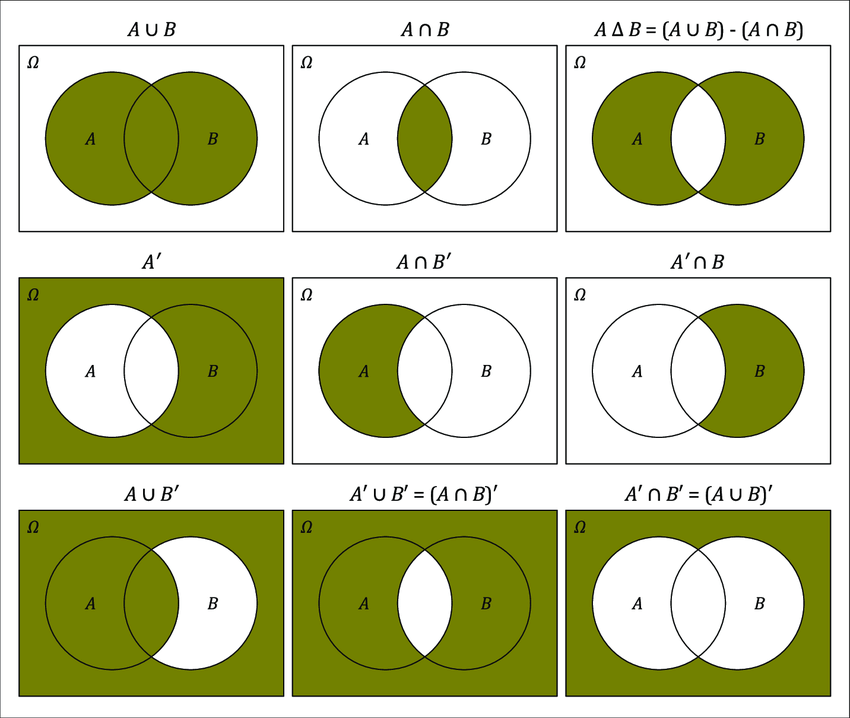
\includegraphics[width=0.7\textwidth]{figures/chapter_5/sets.png}
				\caption{A Venn diagram of unions and intersections for two sets, $A$ and $B$ and their complements, within a universe $\Omega$ $A$,$B$}
				%\source{Sets Graphs and Things We Can See A Formal Combinatorical Ontology for Empirical Intra Site Analysis}
				\label{fig:chap5-sets-1}
			\end{figure}
			\textit{Image taken from listed source\autocite{chap_5_set_figure_1}}\change{Autocite not working for footnote in figure, find a workaround} 
			\\\\
			It should be noted that the set comliment ($A'$) is \textbf{not well defined} in python as it relied on the existance of a universe $\Omega$. We can see how each of these actions actually work by running the following code.

			\lstinputlisting[style=console]{code_examples/chapter_5/set_example_output.txt}


		\section{Dictionary} \label{sec:dictionary}
			This is just an implementation of a more complex datastructure called a hashmap. Hashmaps essentially take a \textbf{key} and associate them with a specific \textbf{value}. To define a dictionary, we do almost hte exact same thing as a set, we use curly brackets (``\{\}''). However, the key difference is we have to define a \textbf{key value pair} where we use a colon (``:'') to seperate the key and the value. If this was a bit hard to understand, I would suggest looking at the example below:
			
			\lstinputlisting[language=python]{code_examples/chapter_5/dictionary_def.py}

			It is worth noting that you dont \textit{have to} put the keys-value pairs on seperate lines, but is general practice.
			
		\section{Advanced Data-structures}
			\subsection{Linked Lists}

			\subsection{Stacks}

			\subsection{Queues}

			\subsection{Trees}
				\subsubsection{Binary Trees}

				\subsubsection{Binary Search Trees}

				\subsection{Heap}

			\subsection{Hashmaps}

			\subsection{Matrix}


	\chapter{Simple Algorithms} \label{chap:simple-algorithms}
		\section{Sorting}
			\subsection{Selection Sort}

			\subsection{Bubble Sort}

			\subsection{Insertion Sort}

			\subsection{Quick Sort}

		\section{Searching}
			\subsection{Linear Search}

			\subsection{Binary Search}

		\section{Intro to Basic Time Complexity}
			This bit may confuse a lot of people. In my opinion, it's definetly one of the harder concepts to pickup and it took me a while to gian an intuition on it. While you don't necessarily need to know this in order to learn how to code, it is quite useful in your coding literacy. This is primarily because when you learn the language of big-O notation, you learn how to read the efficiency of algorithms and, by extention, how to critque your own work and make it better.
			
		
	\chapter{Practicing the basics}	\label{chap:basics-practice}
		In order to get the hang of anything, I believe the best way to go about anything is to practice by actually implementing and applying the things you learnt. Therefore, I have provided a few practice projects in this chapter.
		\section{Calculator}
			Building a basic calculator, in my opionion, will get you well aquainted with the absolute basics of any language. By expanding on calculator base, you can start to learn about more sophisticated features such as functional and even object oriented programming. In the appendix, I have provided my approaches to different design concepts.
			\\\\
			To start with applying conditional logic (``if-statements''), I first want you to take an input 
			asking the user what type of operation they want to do.
			%\lstsinputlisting[language=psuedo]{code_examples/chapter_7/calculator_1.txt}
			\lstinputlisting[language=python]{code_examples/chapter_7/calculator_1.py}
			% \begin{algorithm}
			% 	number1 = \texttt{INPUT:} ``Input your first number'' \\
			% 	number2 = \texttt{INPUT:} ``Input your second number'' \\
			% 	operation = \texttt{INPUT:} ``What type of operation do you want to do: Add(1), Subtract(2), Multiply(3), or Divide(4)?'' \\
			% 	\eIf{operation=1}{
			% 		answer = $\text{number1} + \text{number2}$
			% 	} \eIf{operation=2} {
			% 		answer = $\text{number1} - \text{number2}$
			% 	} \eIf{operation=3} {
			% 		answer = $\text{number1} \times \text{number2}$
			% 	} \eIf{operation=2} {
			% 		answer = $\text{number1} \div \text{number2}$
			% 	} {
			% 		\texttt{OUTPUT:} ``Invalid operation''
			% 	}
			% 	\texttt{OUTPUT:} answer
			% \end{algorithm}
		\section{Chatbot}
			
		\section{Management System}
			
		\section{Task Planner}
			
	\chapter{Learning some techniques}  \label{chap:techniques}
		\section{Naming Conventions}

		\section{Error Analysis}

		\section{Packages}
	
	\chapter{Logical Thinking}  \label{chap:logical-thinking}
		One of the most important reasons to learn how to code is logical thinking and breaking down problems. Traditionally, when you're taught how to code, you're like a computer in itself in the sense that your instructor gives you instructions and you are expected to execute them.Q
		\section{Decomposition}
			One of the key ideas on computer science is operationalization or the decomposition of ideas. At the end of the day computer science is about solving problems. Solving a big complicated problem is just that - complicated. Therefore it becomes important that we break down big problems into smaller ones, then break those into even smaller ones, and so on. Essentially, we want a problem so simple that it's almost as easy as writing a function or even a single line of code.
			\\\\
			This is probably the most importnat ideas in learning computer science because it applies to life as a whole. If there is one take away in your learning computer science, let it be this.
			\\\\
			Decomposition is a hard skill to learn, but is not difficult to master. It all boils down to practice. Hence, we will first through the ``theory'' on how to break an idea down. Then go through a few lay examples and then finally finish off with technical examples.
			\\\\
			To \textit{decompose} a problem/system, we need to think of all the smaller problems/systems it's made up of. For example, take the simple equation below.

			\begin{equation*}
				50x + 10 = 60
			\end{equation*}

			Here, to decompose the problem and solve for $x$, we need to do the following operations:

			\begin{enumerate}
				\item Isolate Variable ($x$ should be on one side alone)
				\item Simplify problem
				\item Solve for $x$
			\end{enumerate}
			
			Therefore, we've decomposed the problem. Now lets put this into action

			\begin{align*}
				50x + 10 &= 60 \\
				\text{Step 1}:& \\
				50x + 10 - 10 &= 60 - 10 \\
				\implies 50x &= 60 - 10 \\
				\text{Step 2}:& \\
				\implies 50x &= 50 \\
				\text{Step 3}:& \\
				\implies x &= 1 \\
			\end{align*}
			Hence, we have used decomposition for a simple example. Say now we move on to a more complicated case. \\
			\\
			Say we need to code an alarm clock. There are a lot of functionality we need to think about. A good exercise is to give this a shot yourself before reading further. \toadd{add checkpoints along the way \textit{through} each example to link the importnat idea (decomponsing/operationalizing ideas)}

			\subsection{Alarm Clock Example}
				Say we have an alarm clock. At a high level, an alarm clock must perform the following functions:
				\begin{itemize}
					\item Alarm
					\item Time
				\end{itemize}

				These can further be decomposed into the following
				
				\begin{itemize}
					\item Alarm 
						\begin{itemize}
							\item Sound Alarm
							\item Change Alarm Time
							\item Snooze Alarm
							\item Alarm Volume
						\end{itemize}
					\item Time
						\begin{itemize}
							\item Show Time
							\item Change Time
							\item Update Time (every minuete)
						\end{itemize}
				\end{itemize}

				This should be enough for us to start writing our code. However, say these smaller tasks are still to complicated, we can go ahead and start decomposing these smaller problems even more:
				\begin{itemize}
					\item Alarm 
						\begin{itemize}
							\item Sound Alarm
								\begin{itemize}
									\item Compare current time to alarm time
									\item Send output to activate speaker to start alarm
									\item Get button input to stop alarm
								\end{itemize}
							\item Change Alarm Time
								\begin{itemize}
									\item Get Button Input
									\item Get dial input to change time
									\item Set dial input and change alarm time internally
									\item Lock alarm time until changed again
								\end{itemize}
							\item Snooze Alarm
								\begin{itemize}
									\item $\cdots$
								\end{itemize}
							\item Alarm Volume
								\begin{itemize}
									\item $\cdots$
								\end{itemize}
						\end{itemize}
					\item Time
						\begin{itemize}
							\item Show Time
								\begin{itemize}
									\item $\cdots$
								\end{itemize}
							\item Change Time
								\begin{itemize}
									\item $\cdots$
								\end{itemize}
							\item Update Time (every minuete)
							\begin{itemize}
								\item $\cdots$
							\end{itemize}
						\end{itemize}
				\end{itemize}

				And we can continue doing this on and on until we get to a set of tasks which are easy enough for us to solve and implement directly. \\
				\\
		\subsection{Morning Routine Example}
			Now lets do another example unrelated to Mathematics or Computer Science. Say we need to organize our daily routine and make an indepth checklist as to what we need to do.
			\begin{itemize}
				\item Wake Up
				\item Organize Room
				\item Get Ready
				\item Eat Breakfast
				\item Leave for work/school
			\end{itemize}
			These are our high-level tasks, now lets decompose them:
			\begin{itemize}
				\item Wake Up
					\begin{itemize}
						\item Set alarm the night before
						\item Open eyes, turn on lights
						\item Get out of bed
						\item Turn off alarm
						\item Don't go back to sleep (I struggle with this one some times)
					\end{itemize}
				\item Organize Room
					\begin{itemize}
						\item Make bed
						\item Put out clothes for the day
						\item Collect daily items (i.e. bag)
					\end{itemize}
				\item Get Ready
					\begin{itemize}
						\item Go to bathroom and take a shower
						\item Dry off and put on clothes
						\item Put on socks and shoes
					\end{itemize}	
				\item Eat Breakfast
					\begin{itemize}
						\item Make breakfast
						\item Get utensils
						\item Make coffee
						\item Eat food that your made
						\item Drink coffee
					\end{itemize}
				\item Leave for work/school
			\end{itemize}

			Notice that there are still some tasks which may not be simple enough while there are others which are just at the right level of simplificiation. Hence, let's do one more decomposition pass.
		
			\begin{itemize}
				\item Wake Up
					\begin{itemize}
						\item Set alarm the night before
						\item Open eyes, turn on lights
						\item Get out of bed
						\item Turn off alarm
						\item Don't go back to sleep (I struggle with this one some times)
					\end{itemize}
				\item Organize Room
					\begin{itemize}
						\item Make bed
							\begin{itemize}
								\item Flatten base cover
								\item Retuck sheet
								\item Fold duvet and place at foot of bed
								\item Put pillows at head of bed 
								\item Organize any other misc items
							\end{itemize}
						\item Put out clothes for the day
						\item Collect daily items (i.e. bag)
							\begin{itemize}
								\item Get wallet
								\item Get phone
								\item Pack bag (if not already packed)
								\item Get bag
								\item Get keys
								\item Get jacket (if going to rain or raining)
							\end{itemize}
					\end{itemize}
				\item Get Ready
					\begin{itemize}
						\item Go to bathroom and take a shower
						\item Dry off and put on clothes
						\item Put on socks and shoes
					\end{itemize}	
				\item Eat Breakfast
					\begin{itemize}
						\item Make Breakfast
							\begin{itemize}
								\item Decide on breakfast (say eggs with toast)
								\item Get pan
								\item Heat up pan
								\item Get eggs
								\item Get spices
								\item Get oil
								\item Put oil in pan
								\item Put eggs in pan
								\item Add spices
								\item Cook eggs as desired
								\item Get plate
								\item Put eggs on plate
								\item Get toaster
								\item Put toast in toster
								\item Put toast on plate
							\end{itemize}
						\item Get utensils
						\item Make coffee
						\item Eat food that your made
						\item Drink coffee
					\end{itemize}
				\item Leave for work/school
			\end{itemize}

			Notice that as we decompose some of our steps start to look like steps. That means we're transitioning from breaking down our problem to actually solving it. Hence, in the above example, the ``Make breakfast'' tasks would actually be better suited to \hyperref[sec:psuedocode]{\texttt{psuedocode}} or a \hyperref[sec:flowchart]{\texttt{flowchart}}, both of which we will explore in the next section.

		\section{Planning}
			We can now take this idea of decomposition further and use it in planning. There are two primary ``formal'' methods we will cover - Psuedocode and Flowcharts. Both are important in different ways. The former allows use to \textit{specifically} write out the logic of our code and how it works without committing it to a specific language instead being written in an English-adjacent language called pseudocode. While there are no universally specific guidelines for writing psuedocode, I will outline some traditionally accepted practices.
			\\\\
			Flowcharts on the other hand allow us to \textit{generally} write out the logic of our code. That is to say, we can more holistically see how are code works from a higher level. This allows others (and us) to understand how are code works. It also helps with the idea of decomposition which was covered in the previous section.
			\\\\
			The overall objective of this chapter is to give you and introduction to both of these planning tools. Probably they're most important purpose is not solely helping you understand your code more but also helping others understand your work. Therefore, these methods greatly help with collaboration on bigger projects (which to many people's disdain, you're probably going to have to do eventually if you plan on doing almost anything meaningful).
			
			\subsection{Psuedocode} \label{sec:psuedocode}
			
			\subsection{Flowcharts} \label{sec:flowchart}
				
		\section{Mathematics}
			As with anthing in almost anything STEM, mathematics plays a huge role in computer science. While at the top level, you don't need to deal with a lot of it, I do still think that some of the basics are worth learning as they can come in handy later on. The primary thing that's worth learning is some introduction to logic. While this can get very complicated, we will only touch upon the basics of it here (with provided resources listed). First, lets define some symbols. 
			
			\begin{table}[H]
				\centering
				\begin{tabular}{c|c|c}
					Logic Symbol & Name & Description \\
					\hline
					$\lnot$ & \texttt{NOT} & The ``negation'' of a boolean statement \\
					$\land$ & \texttt{AND} & The conjunction of two boolean functions/statements \\
					$\lor$ & \texttt{OR} & The disjunction of two boolean functions/statements
				\end{tabular}
			\end{table}

			Note that we've introdued some fancy terminology in the table above. The negation of a statement is the opposite of what it says. If something is true, its negation will be false (and vice versa). \\
			\begin{figure}
				\centering
				\begin{minipage}{0.7\linewidth}
					\begin{table}[H]
						\centering
						\begin{tabular}{c|c|c}
							x & $\lnot x$ \\
							\hline
							1 & 0 \\
							0 & 1
						\end{tabular}
					\end{table}
				\end{minipage}
				\begin{minipage}{0.29\linewidth}
					\centering
					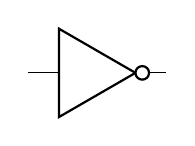
\begin{tikzpicture}
						\ctikzset{logic ports = ieee}
						\node[not port] (Noa) at (0,0){};
					\end{tikzpicture}
				\end{minipage}
			\end{figure}
			Note that in the truth table above, we've used $1=\texttt{TRUE}$ and $0 = \texttt{FALSE}$ as is sometimes is used. We can also write this as a \textit{logic gate} which is a more computer science approach and is a more visual approach to how truth tables and logic works. \\
			\\
			The conjunction of a statement is true if (and only if) each statement is true.
			\begin{figure}
				\centering
				\begin{minipage}{0.7\linewidth}
					\begin{table}[H]
						\centering
						\begin{tabular}{c|c|c}
							x & y & $x\land y$ \\
							\hline
							0 & 0 & 0 \\
							0 & 1 & 0 \\
							1 & 0 & 0 \\
							1 & 1 & 1
						\end{tabular}
					\end{table}
				\end{minipage}
				\begin{minipage}{0.29\linewidth}
					\centering
					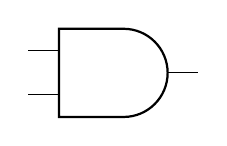
\begin{tikzpicture}
						\ctikzset{logic ports = ieee}
						\node[and port] (ANDa) at (0,0){};
					\end{tikzpicture}
				\end{minipage}
			\end{figure}
			The disjunction of a statement is true if (and only if) any of its statements are true.
			\begin{figure}
				\centering
				\begin{minipage}{0.7\linewidth}
					\begin{table}[H]
						\centering
						\begin{tabular}{c|c|c}
							x & y & $x\lor y$ \\
							\hline
							0 & 0 & 0 \\
							0 & 1 & 1 \\
							1 & 0 & 1 \\
							1 & 1 & 1
						\end{tabular}
					\end{table}
				\end{minipage}
				\begin{minipage}{0.29\linewidth}
					\centering
					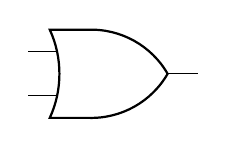
\begin{tikzpicture}
						\ctikzset{logic ports = ieee}
						\node[or port] (ORa) at (0,0){};
					\end{tikzpicture}
				\end{minipage}
			\end{figure}

			Understanding these statements is part of the fundementals of how computers work. As discussed in \ref{sec:computers-binary} everything in a computer is a 1 or 0. Like we did above, this is just a true or a false. Logic gives us the tools to abstractify binary operations and come up with a much more sophisticated approach to problems.

	\chapter{Two Camps}  \label{chap:intro-functional-oops}
		\section{Functional}
			% Avi has offered to write a ``Guest section'' (whatever the fuck that mean)
			\toadd[inline]{Avi's Guest Section}
		\section{Object Oriented}
			
	\chapter{Functional Programming Crash Course} \label{chap:crash-functional}
		% Avi has offered to write a ``Guest chapter'' (whatever the fuck that mean)
		\toadd[inline]{Avi's Guest Chapter}
		\unsure[inline]{FUNC: Maybe remove this from the book and add to follow-up. This seems a bit out of the scope of what's required}
	\chapter{Object Oriented Programming Crash Course} \label{chap:oops}
		\unsure[inline]{OOPS: Maybe remove this from the book and add to follow-up. This seems a bit out of the scope of what's required}
	\section{Classes, Methods, and Objects}
			
		\section{Inheritance}
			
		\section{Encapsulation}
			
		\section{Abstraction}
			
		\section{Polymorphism}
		
	\chapter{Hello World!} \label{chap:hello-world}
		\section{Where do I go from here?}
			Aftering going through this book you should be well equiped to tackle any basic to intermediate programming problems that come your way. That being said, a lot of learning how to code relies on practice and familiarity. 
		\section{Topic/resources to look into (by subject area)}
			\subsection{Algorithms and Mathematics}
				\subsubsection{Formal Logic}
				
				\subsubsection{Linear Algebra}
					\paragraph{Linear Algebra Done Right (S. Axler):} 
						Linear Algebra Done Right by Sheldon Axler is a great book for developing a good foundation in linear algebra. I believe this is the one area of mathematics which is crucial to a good understanding of compuer science. The primary shortcoming of this text is Axler does not go very indepth into determinents (by design), however, I believe this leads to a more solid understanding of the important aspects. You can find Axler's website\footnote{\href{https://linear.axler.net/}{https://linear.axler.net/}} which contains links to buy a copy of the textbook.

					\paragraph{Linear Algebra (J. Hefferon):} 
						I have not personally used this book but I've seen it reccomend quite a bit. The main draw is that this textbook (and question set) are completely free to use. Dr. Hefferon also has a few other books availible for free on his website (which I would highly reccomend checking out).
					
			\subsection{Networking}
				
			\subsection{Data Analysis}
				Sentdex
	\appendix 
	\chapter{Bibliography and References} \label{chap:apdx-bib}
		\printbibliography[heading=none]
	\chapter{Suplemental Code} \label{chap:apdx-sup-code}
\end{document}s